
\documentclass[11pt, a4paper]{book}
\usepackage{svn-multi}
\svnid{$Id$}
\usepackage{prelim2e}
\renewcommand{\PrelimWords}{Draft Copy \svnkw{Id}}
%%\newcommand*{\mysvnrev}{\svnrev}
\usepackage[hyperindex=true,
			bookmarks=true,
            pdftitle={}, pdfauthor={Xi Yang},
            colorlinks=false,
            pdfborder=0,
            pagebackref=false,
            citecolor=blue,
            plainpages=false,
            pdfpagelabels,
            pagebackref=true,
            hyperfootnotes=false]{hyperref}
\usepackage[all]{hypcap}
\usepackage[palatino]{anuthesis}
\usepackage{afterpage}
\usepackage{graphicx}
\usepackage{thesis}
\usepackage[utf8]{inputenc}
\usepackage[square]{natbib}
\usepackage[normalem]{ulem}
\usepackage[table]{xcolor}
\usepackage{makeidx}
\usepackage{cleveref}
\usepackage[centerlast]{caption2}
\usepackage{float}
\urlstyle{sf}
\renewcommand{\sfdefault}{uop}
\usepackage[T1]{fontenc}
\usepackage[scaled]{beramono}

\usepackage{multirow}


\renewcommand*{\backref}[1]{}
\renewcommand*{\backrefalt}[4]{
  \ifcase #1 %
    %
  \or
    (cited on page #2)%
  \else
    (cited on pages #2)%
  \fi
}




%      $Id: macros.tex 506 2009-10-05 16:57:07Z daniel $    

\usepackage{booktabs}
\usepackage{relsize}
\usepackage{xspace}
\usepackage{subfigure}
\usepackage{listings}
\lstloadlanguages{java}
\DeclareGraphicsRule{*}{pdf}{*}{}
\newcommand{\otoprule}{\midrule[\heavyrulewidth]}
\newcommand{\pldi}{ACM Programming Language Design and Implementation (PLDI)}
\newcommand{\taco}{ACM Transactions on Architecture and Code Optimization (TACO)}
\newcommand{\lctes}{ACM Languages, Compiler, and Tool Support for Embedded Systems (LCTES)}
\newcommand{\popl}{ACM Principles of Programming Languages (POPL)}
\newcommand{\ecoop}{European Conference for Object-Oriented Programming (ECOOP)}
\newcommand{\asplos}{ACM Architectural Support for Programming Languages and Operating Systems (ASPLOS)}
\newcommand{\sigmetrics}{ACM Measurement and Modeling of Computer Systems (SIGMETRICS)}
\newcommand{\oopsla}{ACM Object-Oriented Programming, Systems, Languages, and Applications (OOPSLA)}
\newcommand{\ismm}{International Symposium on Memory Management (ISMM)}
\newcommand{\veee}{ACM/USENIX Virtual Execution Environments (VEE)}
\newcommand{\micro}{ACM/IEEE International Symposium on Microarchitecture}
\newcommand{\isca}{ACM/IEEE International Symposium on Computer Architecture (ISCA)}
\newcommand{\icse}{International Conference  on Software Engineering (ICSE)}
\newcommand{\pact}{Parallel Architectures and Compilation Techniques (PACT)}
\newcommand{\casess}{ACM Compilers, Architectures, and Synthesis for Embedded Systems (CASES)}

\definecolor{tableheadcolor}{rgb}{0.8,0.8,1.0}
%\definecolor{tablealtcolor}{rgb}{0.9,0.9,1.0}
\definecolor{tablealtcolor}{rgb}{0.9,0.9,0.95}


\definecolor{todocolor}{rgb}{0.8,0.8,1.0}
\definecolor{fixcolor}{rgb}{1,0.8,0.8}
\definecolor{commentcolor}{rgb}{0.8,1.0,0.8}


\newcommand{\listingfigure}[3]{
\begin{figure}[ht!]
  \begin{center}
    \begin{minipage}[t]{\textwidth-4cm}
      \lstinputlisting{#1}
    \end{minipage}
  \end{center}
  \caption{#3}#2
\end{figure}}

\newcommand{\includeabchart}[5]{
\begin{figure}[ht!]
\begin{center}
\newcommand{\atitle}{#4}
\newcommand{\btitle}{#5}
\input{charts/#1.tex}
\end{center}
\caption{#3}#2
\end{figure}}

\newcommand{\placeholderfigure}[2]{
\begin{figure}[ht!]
  \begin{center}
    \resizebox{\textwidth-2cm}{0.7\textwidth-1.4cm}{todo}
  \end{center}
  \caption{#2}#1
\end{figure}}

\newcommand{\singlegraphfigure}[3]{
\begin{figure}[ht!]
  \begin{center}
    \includegraphics[width=\textwidth-2cm]{#1}
  \end{center}
  \caption{#3}#2
\end{figure}}

\usepackage[color=todocolor, colorinlistoftodos]{todonotes}

%\newcommand{\notinpart}{%
% \def\toclevel@chapter{-1}\def\toclevel@section{0}\def\toclevel@subsection{1}} \newcommand{\inpart}{
% \def\toclevel@chapter{0}\def\toclevel@section{1}\def\toclevel@subsection{2}}


%
% Stuff for pretty printing the source code using listings.sty
%


%% set Java as the default language
\lstset{
  numbers=left,
  numberstyle=\tiny,
  stepnumber=1,
  numbersep=2em,
  language=java,                         % the language
  basicstyle=\footnotesize\ttfamily,     % the basic font family to use
  commentstyle=\itshape,                 % the font for comments
  stringstyle=\ttfamily,
%  morekeywords={@Intrinsic, @Unboxed, @RawStorage}
}
%\lstset{language=java}

\newcommand{\textjava}[1]{{\lstset{basicstyle=\ttfamily}\lstinline@#1@}}
\newcommand{\textjavafn}[1]{{\lstset{basicstyle=\footnotesize\ttfamily}\lstinline@#1@}}
%\usepackage{lstasm}
\usepackage{setspace}
\usepackage{ifthen}
%\usepackage{color}
%\usepackage{smallheadings}

\long\def\sfootnote[#1]#2{\begingroup%
\def\thefootnote{\fnsymbol{footnote}}\footnote[#1]{#2}\endgroup}
%
% code
%

\newcommand{\address}{\textjava{Address}\xspace}
\newcommand{\ubregion}{\textjava{unbump-region()}\xspace}
\newcommand{\word}{\textjava{Word}\xspace}
\newcommand{\freeme}{\textjava{free()}\xspace}
\newcommand{\freemeunbump}{\textjava{unbump()}\xspace}
\newcommand{\freemeunbumpregion}{\textjava{unbump-region()}\xspace}
\newcommand{\freemeunreserve}{\textjava{unreserve()}\xspace}

%
% abbreviations
%


\newcommand{\eg}{e.g., }
\newcommand{\ie}{i.e., }

\newcommand{\GenMS}{\emph{GenMS}\xspace}
\newcommand{\GenImmix}{\emph{GenIX}\xspace}
\newcommand{\mmtk}{MMTk\xspace}
\newcommand{\jikes}{Jikes RVM\xspace} 
\newcommand{\jikesrvm}{\jikes} 
\newcommand{\jala}{Jalape\~{n}o\xspace} 
\newcommand{\jalapeno}{Jalape\~{n}o\xspace} 

\newcommand{\dacapo}{\textsf{DaCapo}\xspace}
\newcommand{\specjvm}{\textsf{SPECjvm98}\xspace}
\newcommand{\cattrack}{\textsf{cattrack}\xspace}
\newcommand{\spec}{\textsf{SPEC}\xspace}

\newcommand{\nurserytype}[1]{{\fontfamily{cmss}\selectfont \textsl{#1}}}
\newcommand{\alloc}{\nurserytype{allocate}\xspace}
\newcommand{\collect}{\nurserytype{collect}\xspace}
\newcommand{\redirect}{\nurserytype{redirect}\xspace}

\newcommand{\bmtype}[1]{{\textsf{#1}}}

\newcommand{\jbb}{\bmtype{jbb2000}\xspace}
\newcommand{\psjbb}{\bmtype{pjbb2005}\xspace}
\newcommand{\pjbb}{\bmtype{pjbb2005}\xspace}
\newcommand{\specjbb}{\bmtype{SPECjbb2005}\xspace}
\newcommand{\jess}{\bmtype{jess}\xspace}
\newcommand{\raytrace}{\bmtype{raytrace}\xspace}
\newcommand{\db}{\bmtype{db}\xspace}
\newcommand{\javac}{\bmtype{javac}\xspace}
\newcommand{\jack}{\bmtype{jack}\xspace}
\newcommand{\compress}{\bmtype{compress}\xspace}
\newcommand{\mpegaudio}{\bmtype{mpegaudio}\xspace}
\newcommand{\mtrt}{\bmtype{mtrt}\xspace}
\newcommand{\antlr}{\bmtype{antlr}\xspace}
\newcommand{\bloat}{\bmtype{bloat}\xspace}
\newcommand{\chart}{\bmtype{chart}\xspace}
\newcommand{\eclipse}{\bmtype{eclipse}\xspace}
\newcommand{\fop}{\bmtype{fop}\xspace}
\newcommand{\hsqldb}{\bmtype{hsqldb}\xspace}
\newcommand{\jython}{\bmtype{jython}\xspace}
\newcommand{\luindex}{\bmtype{luindex}\xspace}
\newcommand{\lusearch}{\bmtype{lusearch}\xspace}
\newcommand{\Lusearch}{\bmtype{Lusearch}\xspace}
\newcommand{\pmd}{\bmtype{pmd}\xspace}
\newcommand{\ps}{\bmtype{ps}\xspace}
\newcommand{\SPECjbb}{\bmtype{SPECjbb}\xspace}
\newcommand{\xalan}{\bmtype{xalan}\xspace}
\newcommand{\sunflow}{\bmtype{sunflow}\xspace}
\newcommand{\Sunflow}{\bmtype{Sunflow}\xspace}
\newcommand{\avrora}{\bmtype{avrora}\xspace}
\newcommand{\core}{Core2 Quad\xspace}
\newcommand{\corelong}{Intel Core2 Quad Q6600\xspace}
\newcommand{\phenom}{Phenom II\xspace}
\newcommand{\phenomlong}{AMD Phenom II X6 1055T\xspace}
\newcommand{\sandy}{i7-2600\xspace}
\newcommand{\sandylong}{Intel Core i7-2600\xspace}



\newcommand{\ghostscript}{\bmtype{ghostscript}\xspace}

\newcommand{\doi}[1]{\href{http://dx.doi.org/#1}{\nolinkurl{doi:#1}}}
%
% misc
%
\newcommand{\fix}[1]{\todo[color=fixcolor]{#1}}
\newcommand{\comment}[1]{\todo[color=commentcolor]{#1}}
\newcommand{\ifix}[1]{\todo[inline,color=fixcolor]{#1}}
\newcommand{\icomment}[1]{\todo[inline,color=commentcolor]{#1}}
\newcommand{\itodo}[1]{\todo[inline]{#1}}
\newcommand{\ignore}[1]{}
\newcommand{\mccenter}[1]{\multicolumn{1}{c|}{#1}}

%
% figure spacing
%
%\clubpenalty 10000
%\widowpenalty 10000
%\def\topfraction{0.9}
%\def\bottomfraction{0.9}
%\def\textfraction{0.1}
%\renewcommand{\singlespacing}{\renewcommand{\baselinestretch}{1.00}\small\normalsize}
%\renewcommand{\doublespacing}{\renewcommand{\baselinestretch}{1.5}\small\normalsize}
%\newcommand{\tight}{\renewcommand{\baselinestretch}{1.28}\small\normalsize}
%\renewcommand{\subfigbottomskip}{0.25ex}
%\renewcommand{\subfigcapskip}{0ex}
%\renewcommand{\subfigcapskip}{-1ex}
%\newcommand{\subfigshrink}{-0.75ex}
%\newcommand{\subfigcapspace}{2ex}

%\newcommand{\subwidth}[0]{.32\textwidth}


%
% margins
%
%\topmargin -.5truein
%\textheight 9truein
%\oddsidemargin .25truein
%\evensidemargin .25truein
%\textwidth 6truein


%
% crossreferencing footnotes
%
%\newcommand{\fnref}[1]{~(\ref{#1})}
%\newcommand{\onecolparbox}{3.1in}


%\newcommand{\textjava}[1]{{\lstset{language=java,basicstyle=\footnotesize\ttfamily}\lstinline@#1@}}
%\newcommand{\textasm}[1]{{\lstset{language=asm,basicstyle=\footnotesize\ttfamily}\lstinline@#1@}}

%%
%% Change the sections etc.
%%
%\makeatletter
%\parskip=0pt
%\renewcommand\section{\@startsection{section}{1}{\z@}%
%                                   {-2.5ex}% beforeskip
%%                                   {1ex}% afterskip
%                                   {\large \bfseries \raggedright}}
% \renewcommand\subsection{\@startsection{subsection}{2}{\z@}%
%                                     {-2ex\@plus -1ex \@minus -.2ex}%
%                                      {.5ex \@plus .2ex}%
%                                      {\normalsize \bfseries \raggedright}}
% \renewcommand\subsubsection{\@startsection{subsubsection}{3}{\z@}%
%                                      {-2ex\@plus -1ex \@minus -.2ex}%
%                                      {1ex \@plus .2ex}%
%                                      {\normalfont\fontsize{11pt}{12pt}\selectfont\itshape}}
%\renewcommand{\thesubsubsection}{\thesubsection.\arabic{subsubsection}}

%\renewcommand\paragraph{\@startsection{paragraph}{4}{\z@}% 
%  {.5em}%
%  {-1em}%
%  {\normalfont\normalsize\bfseries\parskip=0pt}}
%\setlength\partopsep{0\p@}
%\setlength\parskip{0\p@ \@plus \p@}

%\makeatother
%\parindent=9pt





%%% Local Variables: 
%%% mode: latex
%%% TeX-master: "doa"
%%% End:
            
%%%%%%%%%%%%%%%%%%%%%%%%%%%%%%%%%%%%%%%%%%%%%%%%%%%%%%%%%%%%%%%%%%%%%%%
%% Preamble
\title{Applying Context-Tree Weighting To Learning in Various Environments}
\author{John Aslanides, 
 Ryk Budzynski,
 Jarryd Martin, 
 Nrupenda Rao, 
 Yadunandan Sannappa, 
 Cheng Yu}
\date{20 October, 2015}

\renewcommand{\thepage}{\roman{page}}

\makeindex
\begin{document}
%\doparttoc
%%%%%%%%%%%%%%%%%%%%%%%%%%%%%%%%%%%%%%%%%%%%%%%%%%%%%%%%%%%%%%%%%%%%%%%
%% Title page
\pagestyle{empty}
\thispagestyle{empty}
%% anuthesis.sty Copyright (C) 1996, 1997 Steve Blackburn
%% Department of Computer Science, Australian National University
%%

\begin{titlepage}
  \enlargethispage{2cm}
  \begin{center}
    \makeatletter
    \Huge\textbf{\@title} \\[.4cm]
    \Huge\textbf{\thesisqualifier} \\[2.5cm]
    \huge\textbf{\@author} \\[9cm]
    \makeatother
%%   \LARGE A thesis submitted for the degree of \\
%%    Master of Philosophy at \\
%%    The Australian National University \\[2cm]
    \LARGE A thesis submitted for the degree of \\
    YOUR DEGREE NAME \\
    The Australian National University \\[2cm]
    \thismonth
  \end{center}
\end{titlepage}


%%%%%%%%%%%%%%%%%%%%%%%%%%%%%%%%%%%%%%%%%%%%%%%%%%%%%%%%%%%%%%%%%%%%%%%
%% Here begin the preliminaries
\vspace*{14cm}
\begin{center}
  \makeatletter
  \copyright\ \@author{} 2011
  \makeatother
\end{center}
\noindent
\begin{center}
  \footnotesize{~} %\aboutthesis
\end{center}
\noindent

\newpage

\vspace*{7cm}
\begin{center}
  Except where otherwise indicated, this thesis is my own original
  work.
\end{center}

\vspace*{4cm}

\hspace{8cm}\makeatletter\@author\makeatother\par
\hspace{8cm}\today


%%%%%%%%%%%%%%%%%%%%%%%%%%%%%%%%%%%%%%%%%%%%%%%%%%%%%%%%%%%%%%%%%%%%%%%
%% Dedication
\cleardoublepage
\pagestyle{empty}
\vspace*{7cm}
\begin{center}
to my xxx, yyy (yyy is the people you want to dedicated this thesis to.)
\end{center}


%%%%%%%%%%%%%%%%%%%%%%%%%%%%%%%%%%%%%%%%%%%%%%%%%%%%%%%%%%%%%%%%%%%%%%%
%% Acknowledgements
\cleardoublepage
\pagestyle{empty}
\chapter*{Acknowledgments}
\addcontentsline{toc}{chapter}{Acknowledgments}
Who do you want to thank?


%%%%%%%%%%%%%%%%%%%%%%%%%%%%%%%%%%%%%%%%%%%%%%%%%%%%%%%%%%%%%%%%%%%%%%%
%% Abstract
\cleardoublepage
\pagestyle{headings}
\chapter*{Abstract}
\addcontentsline{toc}{chapter}{Abstract}
\vspace{-1em}
Put your abstract here.

%%% Local Variables: 
%%% mode: latex
%%% TeX-master: "paper"
%%% End: 

%%%%%%%%%%%%%%%%%%%%%%%%%%%%%%%%%%%%%%%%%%%%%%%%%%%%%%%%%%%%%%%%%%%%%%%
%% Table of contents
\cleardoublepage
\pagestyle{headings}
\markboth{Contents}{Contents}
\tableofcontents
\listoffigures
\listoftables

%%%%%%%%%%%%%%%%%%%%%%%%%%%%%%%%%%%%%%%%%%%%%%%%%%%%%%%%%%%%%%%%%%%%%%
%% Here begins the main text
\mainmatter

%% Introduction
\chapter{Introduction}
\label{cha:intro}
Hutter has proven that AIXI model produces better result than any other existing learning algorithm. The Bayesian Mixture model will converge to the unknown true model.  However, Kolmogorov complexity is incomputable. Using Context Tree Weighting and Monte Carlo sampling as approximation, we can build a universal reinforcement learning agent based on approximation of AIXI.

\section{Main Finding}
\label{sec:thesisstatement}
Group 3 has implemented the reinforcement agent that can learn from various encoded environments.


\section{Introduction}
\label{sec:problemstatement}
This assignment is closely related to Veness's paper. We are building a reinforcement learning agent using UCT algorithm, MC sampling, AIXI, and universal Bayesian mixture. The agent then learns to play Pacman, Tic-Tac-Toe, Biased Rock-Paper-Scissor, Extended Tiger, and Cheese Maze. 


\section{Thesis Outline}
\label{sec:outline}
Chapter~\ref{cha:background} mainly deals with the theoretical findings of Vanness' paper, and briefly touches on Monte Carlo sampling, UTC algorithm, context tree weighting [V+11], and how our agent combines these, as required by the assignment.
Chapter~\ref{cha:design}  
Chapter~\ref{cha:methodology},
Chapter~\ref{cha:result}, and Chapter~\ref{cha:conc}.


%% Chapters
\chapter{Background and Related Work}
\label{cha:background}
At the begging of each chapter, please introduce the motivation and high-level
picture of the chapter. You also have to introduce sections in the
chapter. \\


Section~\ref{sec:motivation} xxxx.\\


Section~\ref{sec:relatedwork} yyyy.\\


\section{Motivation}
\label{sec:motivation}


\section{Related work}
\label{sec:relatedwork}
You may reference other papers. For example: 
Generational garbage collection~\citep{LH:83,Moon:84,Ungar:84} is perhaps the
single most important advance in garbage collection since the first collectors
were developed in the early 1960s. (doi: "doi" should just be the doi part, not
the full URL, and it will be made to link to dx.doi.org and resolve.
shortname: gives an optional short name for a conference like PLDI '08.)





\section{Summary}
Summary what you discussed in this chapter, and mention the story in next
chapter. Readers should roughly understand what your thesis takes about by only reading
words at the beginning and the end (Summary) of each chapter.




\chapter{Design and Implementation}
\label{cha:design}
Same as the last chapter, introduce the motivation and the high-level picture to
readers, and introduce the sections in this chapter.


\section{Smart Design}
\label{sec:des-hotpath}

\section{Summary}
Same as the last chapter, summary what you discussed in this chapter and
be the bridge to next chapter.

\chapter{Experimental Methodology}
\label{cha:methodology}

\section{Software platform}
\label{sec:softplat}
We use C++ standard libraries. Due to time and library constraints, we decide not to visualise the cheese maze and pacman. 

See Appendix for implementation documentation including class diagram.


\section{Hardware platform}
\label{sec:hardplat}

Table~\ref{tab:machines} shows how to include tables and Figure~\ref{fig:helloworld} shows how to include codes.
\begin{table*}
  \centering
  \input table/machines.tex
  \caption{Processors used in our evaluation.}
  \label{tab:machines}
\end{table*}



\begin{figure}
  \centering
  \subfigure[\label{fig:c:hello}]{
  \begin{minipage}[b]{\columnwidth}
    \lstinputlisting[linewidth=\columnwidth,breaklines=true]{code/hello.c}\vspace*{-2ex}
  \end{minipage}}
  \subfigure[\label{fig:java:hello}]{
  \begin{minipage}[b]{\columnwidth}
    \lstinputlisting[linewidth=\columnwidth,breaklines=true]{code/hello.java}\vspace*{-2ex}
  \end{minipage}}
  \caption{Hello world in Java and C.}
  \label{fig:helloworld}
\end{figure}




%%% Local Variables: 
%%% mode: latex
%%% TeX-master: "paper"
%%% End: 

\chapter{Results}
\label{cha:result}




\section{Direct Cost}\
\label{sec:direct_cost}

Here is the example to show how to include a figure. Figure~\ref{fig:cost}
includes two subfigures (Figure~\ref{fig:zerocost}, and Figure~\ref{fig:zerobus});

\begin{figure*}
  \label{fig:cost}
  \subfigure[Fraction of cycles spent on zeroing\label{fig:zerocost}]{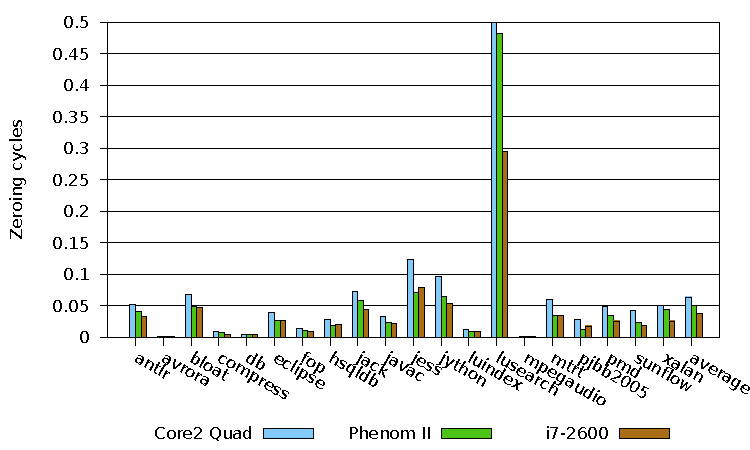
\includegraphics[width=\columnwidth]{figs/zerocost_intel.pdf}}
  \subfigure[BytesZeroed / BytesBurstTransactionsTransferred\label{fig:zerobus}]{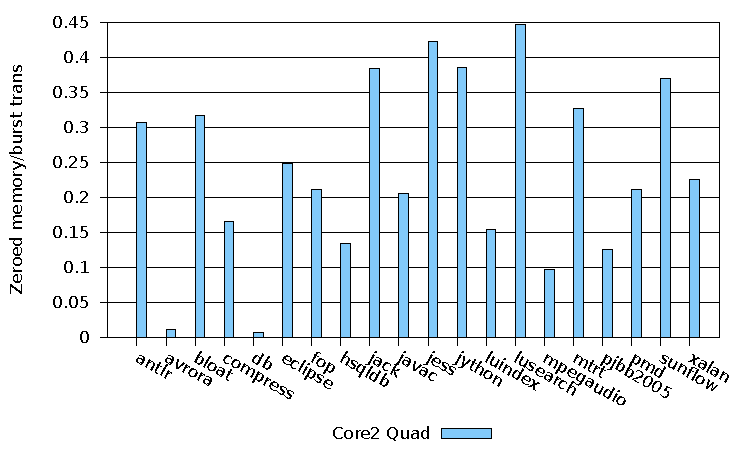
\includegraphics[width=1.0\columnwidth]{figs/zerobus_core.pdf}}
  \caption{The cost of zero initialization}
\end{figure*}


\section{Summary}

\chapter{Conclusion}
\label{cha:conc}
Summary your thesis and discuss what you are going to do in the future in Section~\ref{sec:future}.


\section{Future Work}
\label{sec:future}
Good luck.





%%%%%%%%%%%%%%%%%%%%%%%%%%%%%%%%%%%%%%%%%%%%%%%%%%%%%%%%%%%%%%%%%%%%%%
% Here begins the end matter

% \appendix

\backmatter

\bibliographystyle{anuthesis}
\bibliography{thesis}

\printindex

\end{document}
